%% CAPITULO 1
\hypertarget{estilo:capitulo}{}
\chapter{INTRODUÇÃO} 

\section{Motivação}
\label{ss:motivacao}

A precipitação é um dos principais fenômenos da natureza que exerce grande influência na vida do homem e dos animais. Entende-se por precipitação toda a forma de água proveniente do vapor d'água da atmosfera e depositada sobre a superfície terrestre, como chuva, granizo, orvalho, neblina, neve ou geada \cite{pintoetal76}. A atmosfera atua como um grande reservatório de vapor d'água, o qual transporta e distribui a precipitação no planeta e, toda a água que está depositada sobre a superfície terrestre, é resíduo das precipitações. A precipitação sob a forma de chuva, além de ser mais facilmente medida, é a que mais contribui para a vazão dos rios sobre a América do Sul (AS).

O Ciclo Hidrológico (CH) é um mecanismo da natureza que tem como componente principal a precipitação - \autoref{fig01}. A água que evapora do solo, dos rios e lagos e que é transpirada pela vegetação, aliado ao calor liberado pela transformação física dos estados sólido e líquido da água, são resposáveis pelos mecanismos de formação das nuvens. A convecção, processo físico responsável pela ascenção do vapor d'água presente na atmosfera, transporta o vapor d'água liberado pela superfície, que se consensa formando as nuvens.

\begin{figure}[!hbp]
\centering
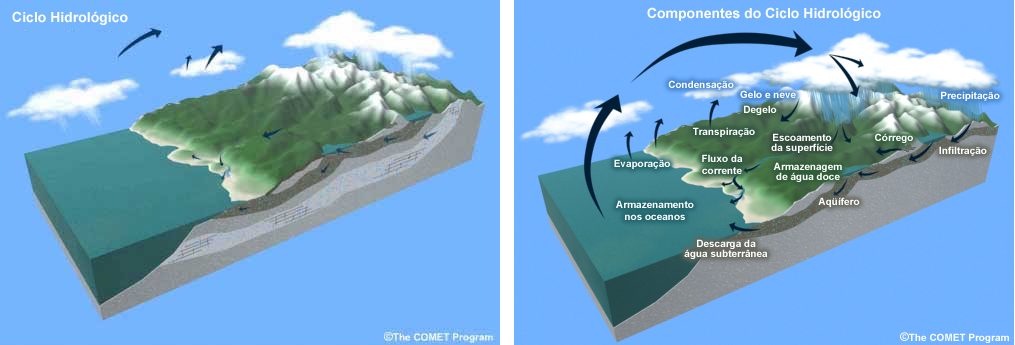
\includegraphics[height=5cm]{./figs/fig01.png}
\caption{Componentes do Ciclo Hidrológico.}
\FONTE{The COMET Program.}
\label{fig01}
\end{figure}

A quantidade, o tipo e a distribuição da precipitação dependem do tipo de nuvem e consequentemente das características do local onde as massas de ar ascendem. Em locais de topografia destacada a precipitação é tipicamente orográfica, caso em que as nuvens são formadas a partir da ascenção forçada do ar sobre as encostas de topografias íngremes. Outro tipo de precipitação, a frontal, é o resultado do encontro de duas massas de ar de características diferentes (de locais diferentes). Há também a precipitação do tipo convectiva, em que as nuvens se formam devido às diferenças de temperatura em uma mesma região. A precipitação do tipo convectiva pode possuir um potencial devastador muito grande, com uma escala de tempo que pode durar desde alguns minutos (em pontos localizados) até horas (em uma determinada região), quando as nuvens que se formam se organizam formando um Sistema Convectivo de Mesoescala (SCM). Estes tipos de nuvens geralmente têm um grande desenvolvimento vertical, podendo chegar a mais de 30 km de altura, desenvolvendo-se ao longo da estratosfera.  Conhecer os diferentes regimes de precipitação - sua distribuição e quantidade sobre uma determinada área ou região, é importante para melhorar o entendimento do CH e de sua interação com as atividades do homem, principalmente sobre a região tropical.

Usualmente, a precipitação é medida nas estações de coleta de dados em superfície através de pluviômetros ou pluviógrafos (aparelhos receptores de água precipitada que registram a altura da água no decorrer do tempo). A precipitação pode também ser estimada através de modelos e radares e, de forma remota, através de satélites - capazes de classificar as nuvens a partir da temperatura de brilho do topo das nuvens. Os radares e os pluviômetros são os principais instrumentos de monitoramento e registro da precipitação. Os radares são importantes porque além de fornecerem informações sobre o posicionamento das nuvens (altura e descolamento horizontal) também podem fornecer informações sobre o tipo de precipitação associada a estas nuvens. Os satélites por sua vez, são poderosos instrumentos capazes de fornecer informações, em tempo real, sobre as condições do fluxo atmosférico em diversas faixas do espectro radiativo e em diversos níveis da atmosfera. No entanto, a quantidade de pluviômetros e radares meteorológicos instalados em superfície, é insuficiente para se determinar de forma acurada a distribuição espacial e temporal da precipitação tropical ao redor do globo. Esta deficiência tem se constituído como um dos problemas mais críticos da meteorologia atualmente.

Nesse sentido, o propósito desta dissertação de mestrado é contribuir com o aprimoramento do sistema de previsão EtaWS+RPSAS do CPTEC (Centro de Previsão de Tempo e Estudos Climáticos) a partir da assimilação de dados de precipitação do satélite TRMM (Tropical Rainfall Measuring Mission). Para tanto, com este trabalho buscou-se atingir os objetivos a seguir.

\section{Objetivos}
\label{ss:objetivos} 

\textbf{Objetivo Geral:}

O objetivo principal deste trabalho é avaliar o impacto da inclusão de dados de precipitação no sistema de assimilação de dados regional do CPTEC. Para este propósito foi utilizado o sistema de assimilação de dados RPSAS junto com o modelo regional de mesoescala EtaWS. Esta avaliação tem também o intuito de verificar como a assimilação de precipitação contribui para o aprimoramento do sistema EtaWS+RPSAS na represetação dos sistemas convectivos.

\textbf{Objetivos Específicos:}

\begin{itemize}
\item Realização de experimentos com e sem assimilação de precipitação;
\item Avaliação do impacto da assimilação de precipitação e avaliação do skill do modelo;
\item Estudo de caso de CCM ocorrido em janeiro de 2003: identificação e simulação (ciclo de vida, posicionamento e intensidade).
\end{itemize}
